\begin{document}

{
    \usebackgroundtemplate{
\includegraphics[width=\paperwidth]{capa.png}}
    \begin{frame}[plain]
        \vspace{18mm}
        \begin{flushright}
        \textcolor{cinza}{\textbf{\large{\thetitle}}}
    \end{flushright}

    \vspace{-6mm}
    \begin{flushright}
        \textcolor{cinza}{\textbf{\scriptsize{\theauthor}}}
    \end{flushright}

    \vspace{-7mm}
    %%%
    %%% Formação | Departamento | Centro
    %%%
    \begin{flushright}
        \textcolor{cinza}{\scriptsize{
            Bacharelado em Ciência da Computação | Informática e Estatística | Centro Tecnológico
        }}
    \end{flushright}


    \end{frame}
}

%%%
%%% Demais slides (exceto o slide final)
%%%
\begin{frame}{Terminologia}
    \begin{itemize}
        \item \textbf{Busca:} Conceito genérico de busca;
        \item \textbf{Consulta:} Processo completo de buscar por processos;
        \item \textbf{Consulta Processual:} Preencher e enviar o formulário de
            consulta processual de um TJ.
    \end{itemize}
\end{frame}

\begin{frame}{Estrutura}
    \tableofcontents
\end{frame}

\section{TJScraper}

\begin{frame}{O que é}
    TJScraper é uma biblioteca e uma aplicação de \textbf{extração} de dados
    processuais de portais públicos dos Tribunais de Justiça Brasileiro.

    \vspace{1em}

    Interfaces:
    \begin{itemize}
        \item Linha de Comando (ILC);
        \item Web.
    \end{itemize}
\end{frame}

\begin{frame}{Organização Geral}
    \begin{figure}[H]
        \centering
        \begin{tikzpicture}[
                scale=0.6,
                transform shape,
                edge from parent path={(\tikzparentnode\tikzparentanchor) |- (\tikzchildnode\tikzchildanchor)},
                % Childs
                module/.style = {grow = down, anchor = west, xshift=1em,
                    edge from parent path={(\tikzparentnode.south) |- (\tikzchildnode.west)},
                },
                category/.style = {},
                % Categories
                level 1/.style = {sibling distance = 8em},
                level 2/.style = {level distance = 5em},
                interface/.style = {grow = down, rectangle, draw, blue, fill=blue!20},
                utils/.style = {grow = down, rectangle, draw, gray, fill=gray!20},
                extract/.style = {grow = down, rectangle, draw, green!50!black, fill=green!20},
            ]
            \node [draw] {tj\_scraper}
                child [grow=down] [edge from parent fork down]
                child [category] {
                    node[utils] {Utilitários}
                        child [module, level distance = 1 * 3em] {node [utils] {.errors}}
                        child [module, level distance = 2 * 3em] {node [utils] {.process}}
                        child [module, level distance = 3 * 3em] {node [utils] {.statistics}}
                        child [module, level distance = 4 * 3em] {node [utils] {.timing}}
                        child [module, level distance = 5 * 3em] {node [utils] {.url}}
                    }
                child [category] {
                    node[interface] {Interface}
                        child [module, level distance = 1 * 3em] {node [interface] {.cli}}
                        child [module, level distance = 2 * 3em] {node [interface] {.webapp}}
                    }
                %[edge from parent fork down]
                child [category] {
                    node[extract] {Extração}
                        child [module, level distance = 1 * 3em] {node [extract] {.cache}}
                        child [module, level distance = 2 * 3em] {node [extract] {.download}}
                        child [module, level distance = 3 * 3em] {node [extract] {.export}}
                        child [module, level distance = 4 * 3em] {node [extract] {.html}}
                    }
                ;
        \end{tikzpicture}
    \end{figure}
\end{frame}

\begin{frame}{ILC}
    \todo{}
\end{frame}

\begin{frame}{Aplicação Web}
    \todo{:)}
\end{frame}

\section{Estratégias de extração}

\subsection{Como descobrir processos}

\begin{frame}{TJ-RJ: Página de Consulta Processual}
\end{frame}

\begin{frame}{Sistemas de Numeração}
    \begin{itemize}
        \item \textbf{Unificada}: Padronizado pelo CNJ. Formato:
            ``NNNNNNN-DD.AAAA.J.TR.OOOO''.
        \item \textbf{Antiga}: Padrão interno de cada TJ. Formato do TJ-RJ:
            ``AAAA.OOO.NNNNNN-N''.
    \end{itemize}
\end{frame}

\subsection{Extração HTML}

\begin{frame}{TJ-RJ: Visualização de Processos}
    \begin{figure}[htb]
        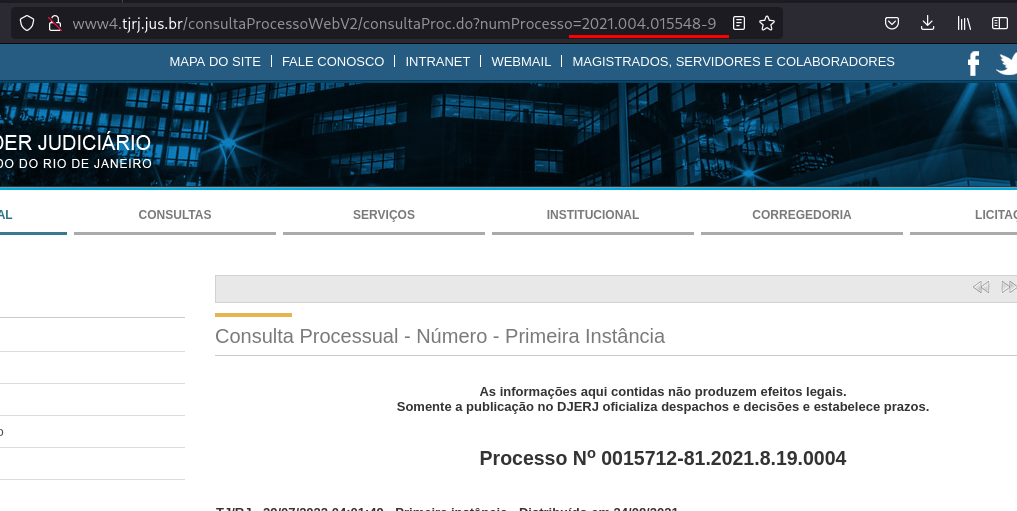
\includegraphics[keepaspectratio,width=1\textwidth]{img/tj-rj-1}
    \end{figure}
\end{frame}

\begin{frame}{TJ-RJ: Visualização de Processos}
    \begin{figure}[htb]
        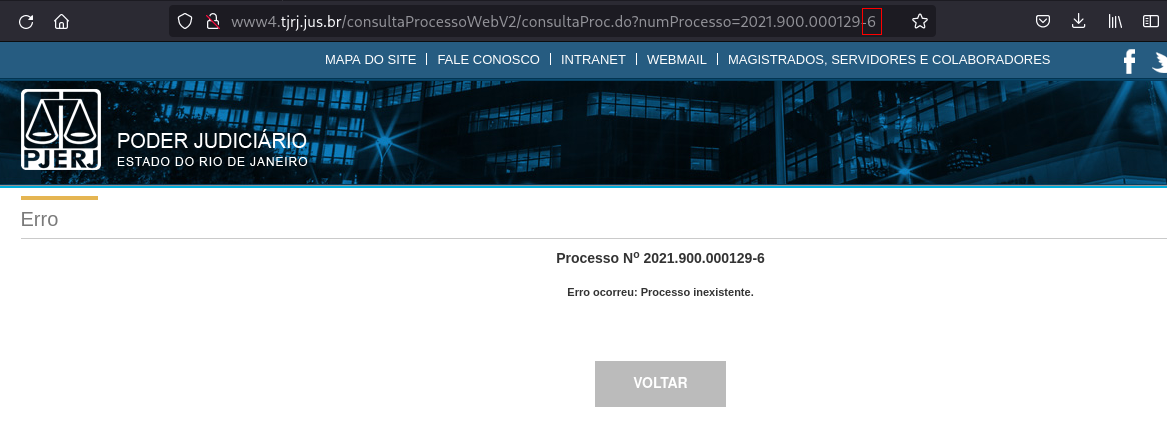
\includegraphics[keepaspectratio,width=1\textwidth]{img/tj-rj-2}
    \end{figure}
\end{frame}

\begin{frame}{Etapas}
    \begin{itemize}
        \item Descoberta de processos via numeração \textbf{antiga};
        \item \textit{Download} de processos;
        \item \textit{Parsing} de HTML;
        \item Exportação de processos.
    \end{itemize}
\end{frame}

\begin{frame}{Scrapy e XPath}
    % Revisitaremos a escolha de Scrapy mais à frente nas conclusões
\end{frame}

\subsection{Extração via API JSON}

\begin{frame}{TJ-RJ: Consulta processual via ww3}
    % Colocar página de busca do ww3
\end{frame}

\begin{frame}{TJ-RJ: Consulta processual via ww3}
    % Colocar logs de Network do navegador
\end{frame}

\begin{frame}{TJ-RJ: Objetos JSON}
    % Mostrar resposta para numeração única (pode ser print do navegador)
    % Mostrar resposta para numeração antiga (pode ser print do navegador)
\end{frame}

\begin{frame}{Etapas}
    \begin{itemize}
        \item Descoberta de processos via numeração \textbf{unificada};
        \item \textit{Download} de processos via numeração \textbf{antiga};
        \item Seleção dos campos desejados;
        \item Exportação de processos.
    \end{itemize}
\end{frame}

\section{Estratégias de Aceleração de Consulta}

\subsection{Requisições Assíncronas}

% TODO: Nesta seção, tentar explicar via diagramas (1) e (2)

\begin{frame}{Requisições Assíncronas}
    % Mostrar só em que ponto se colocariam e como foi implementado
    % (1) O diagrama pode ser uma cópia do que está na monografia
\end{frame}

\begin{frame}{Controle de Tráfego via Lotes}
    % Comentar do uso de semáforos, etc.
    % (2) Aqui o diagrama pode ser um "zoom-out" do diagrama da monografia só
    % que com mais seções, explicitando os lotes.
\end{frame}

\subsection{\textit{Cache} dos processos}

\section{Análise de Experimentos}

\subsection{Configuração Experimental}

\subsection{Resultados Experimentais}

\section{Conclusões e Perspectivas}

\begin{frame}{Conclusões do Trabalho}
\end{frame}

\begin{frame}{``O que fazer?''}
    % Trabalhos Futuros
\end{frame}

%%%
%%% Slide final
%%%
{
    \usebackgroundtemplate{
\includegraphics[width=\paperwidth]{capa.png}}
    \begin{frame}[plain]
        \vspace{15mm}
        \begin{center}
            \textcolor{cinza}{\textbf{Discussões abertas}}
        \end{center}
        \vspace{-6mm}
        \begin{center}
        \textcolor{cinza}{
            \scriptsize{E-mail: jpaulotiz@gmail.com}}
        \end{center}
        \vspace{-6mm}
        \begin{center}
        \textcolor{cinza}{\scriptsize{Telefone: (48) 99153-1404}}
        \end{center}
        \vspace{-6mm}
        \begin{center}
        \textcolor{cinza}{\scriptsize{
            Site: \url{https://github.com/jptiz}
        }}
        \end{center}
    \end{frame}
}

\end{document}

